\documentclass[a4paper,10pt]{article}
\usepackage{graphicx}
\usepackage[russian]{babel}
\usepackage{cmap}
\usepackage[T2A]{fontenc}
\usepackage[utf8]{inputenc}
\usepackage{mathtools}
\usepackage{float}
\usepackage{titlesec}
\usepackage{varioref}
\usepackage{fancyhdr}
\usepackage{multicol}
\usepackage{mathrsfs}
\usepackage{wrapfig}
\usepackage{gensymb}
\usepackage{subcaption}
\usepackage[table]{xcolor}
\usepackage{amsmath}

\begin{document}

\begin{center}
    {\large МОСКОВСКИЙ ФИЗИКО-ТЕХНИЧЕСКИЙ ИНСТИТУТ (НАЦИОНАЛЬНЫЙ ИССЛЕДОВАТЕЛЬСКИЙ УНИВЕРСИТЕТ)}
\end{center}

\vspace{4.5cm}
{\Large
\begin{center}
\end{center}
{\bf Отчёт о выполнении лабораторной работы 3.6.1}\\
Спектральный анализ электрических сигналов
}
\vspace{2cm}
\begin{flushright}
    {\normalsize Галкина Мария, Высоцкая Ирина \\
    \vspace{0.2cm}
    Б03-502}
\end{flushright}
\vspace{8cm}


\section{Аннотация}
\noindent \textbf{Цель работы:} изучить спектры сигналов различной формы и влияние параметров сигнала на вид соответсвтующих спектров; проверить справедливость соотношений неопределенностей; познакомиться с работой спектральных фильтров на примере RC-цепочки.\\
\textbf{В работе используются:} 
генератор сигналов произвольной формы, цифровой осциллограф с функцией быстрого преобразования Фурье или цифровой USB-осциллограф, подключенный к персональному компьютеру.

\section{Теоретические сведения}


\subsection*{Ряд Фурье и спектр сигнала}

Любая периодическая функция с периодом $T$ может быть представлена в виде ряда Фурье:
\begin{equation}
f(t) = \frac{A_0}{2} + \sum_{n=1}^{\infty} A_n \cos(2\pi\nu_n t) + B_n \sin(2\pi\nu_n t),
\end{equation}
где $\nu_n = n\nu_0$, $\nu_0 = 1/T$ --- частоты гармоник, а коэффициенты равны
\begin{equation}
A_n = \frac{2}{T}\int_0^T f(t)\cos(2\pi\nu_n t)\,dt, \qquad
B_n = \frac{2}{T}\int_0^T f(t)\sin(2\pi\nu_n t)\,dt.
\end{equation}
Эквивалентная форма записи в представлении амплитуд и фаз:
\begin{equation}
f(t) = \frac{a_0}{2} + \sum_{n=1}^{\infty} a_n \cos(2\pi\nu_n t + \varphi_n),
\end{equation}
где $a_n = \sqrt{A_n^2 + B_n^2}$, $\operatorname{tg}\varphi_n = B_n/A_n$.

Совокупность частот $\nu_n$ и соответствующих амплитуд $a_n$ (и фаз $\varphi_n$) называют \emph{спектром} функции $f(t)$. Для чётной функции $B_n \equiv 0$ (разложение по косинусам), для нечётной $A_n \equiv 0$ (разложение по синусам).

Спектр периодической функции \emph{дискретен}. Для непериодического (ограниченного во времени) сигнала при $T \to \infty$ расстояние между гармониками $\delta\nu = 1/T \to 0$, и спектр становится \emph{непрерывным} (ряд Фурье переходит в интеграл Фурье).

При спектральном анализе измеряются, как правило, только амплитуды $|a_n|$ (или интенсивности $|a_n|^2$), а информация о фазах теряется, поэтому взаимно-однозначное соответствие между сигналом и амплитудным спектром пропадает.

\subsection*{Соотношения неопределённостей}

Если у сигнала есть характерное время $\Delta t$ (период повторения, длительность импульса и т.п.), то в спектре наблюдается характерный масштаб
\begin{equation}
\Delta\nu \cdot \Delta t \sim 1.
\end{equation}
Конкретный вид зависит от формы сигнала и от того, что понимается под «характерным» временем и «шириной» спектра. Например, для импульса длительностью $\tau$ ширина спектра $\Delta\nu \sim 1/\tau$. Для любого периодического сигнала с периодом $T$ гармоники отстоят друг от друга на точное расстояние $\delta\nu = 1/T$, не зависящее от формы сигнала.

\subsection*{Методы спектрального анализа}

Различают аналоговые (физические) и цифровые (математические) методы. Простейший физический  --- RLC-цепочка, откликающаяся на частоты вблизи резонансной.

Цифровой анализ основан на дискретизации сигнала и алгоритме быстрого преобразования Фурье (БПФ). Две его особенности:
\begin{itemize}
\item \textbf{Частота дискретизации} $\nu_{\text{дискр}}$: нельзя исследовать частоты выше неё; по теореме Котельникова необходимо $\nu < \nu_{\text{дискр}}/2$. Параметр «количество точек» на интервал времени ограничивает спектр сверху.
\item \textbf{Ограниченность «окна»} регистрации $\Delta t$: возникают краевые искажения спектра, для компенсации применяют весовые («оконные») функции. 
\end{itemize}

\subsection*{Спектры конкретных сигналов}

\textbf{Прямоугольные импульсы} (период $T$, длительность $\tau$):
\begin{equation}
\nu_n = \frac{n}{T}, \qquad
|a_n| = \frac{\left|\sin\frac{\pi n\tau}{T}\right|}{\pi n}
= \frac{\tau}{T}\,\frac{|\sin\pi\nu_n\tau|}{\pi\nu_n\tau}.
\end{equation}
Амплитуды сравнивают в относительных единицах, например $|a_n/a_1|$.

\textbf{Амплитудная модуляция} (несущая $\nu_0$, модуляция $\nu_{\text{мод}}$, глубина $m$): сигнал имеет центральную линию на $\nu_0$ и боковые на $\nu_0 \pm \nu_{\text{мод}}$. Глубина модуляции
\begin{equation}
m = \frac{A_{\max} - A_{\min}}{A_{\max} + A_{\min}},
\end{equation}
а отношение амплитуд боковой и основной линий пропорционально $m$ (теоретически $a_{\text{бок}}/a_{\text{осн}} = m/2$).

\textbf{RC-фильтр низких частот}: характерное время $\tau_{RC} = RC$, характерная частота $\nu_{RC} = 1/\tau_{RC}$. Амплитудный коэффициент фильтрации $K(\nu)$ спадает с ростом частоты; экспериментальная зависимость $K(\nu)$ позволяет определить $\tau_{RC}$.

\section{Экспериментальные данные и обработка результатов}

\subsection*{ Исследование спектра периодической последовательности прямоугольных импульсов}

Согласно теории, спектр периодической последовательности прямоугольных импульсов имеет дискретную структуру. Частоты гармоник кратны частоте повторения \(\nu_n = n \nu_{\text{повт}} = n/T\), а их амплитуды описываются огибающей вида \(|a_n| \propto \frac{|\sin(\pi n \tau / T)|}{n}\), где \(\tau\) — длительность импульса. Для качественного наблюдения за изменениями спектра параметры генератора варьировались поочередно.

\subsubsection*{а) Изменение частоты повторения \(\nu_{\text{повт}}\) при фиксированной длительности \(\tau = 50\) мкс}

На рисунках ниже представлены спектры сигнала при фиксированной длительности импульса \(\tau = 50\) мкс и различных частотах повторения: \(\nu_{\text{повт}} = 1\) кГц, \(5\) кГц и \(7\) кГц.

\begin{itemize}
    \item При \(\nu_{\text{повт}} = 1\) кГц расстояние между соседними гармониками минимально, и в пределах экрана умещается большое количество спектральных линий. Спектр выглядит «частым».
    \item При увеличении \(\nu_{\text{повт}}\) до \(5\) кГц и \(7\) кГц расстояние между гармониками \(\delta\nu = 1/T\) заметно увеличивается, и спектр становится более «редким». Количество линий, видимых на экране, уменьшается.
    \item При этом общая огибающая спектра (форма лепестков) и положение частот, на которых амплитуда обращается в ноль, не меняются, так как они определяются исключительно длительностью импульса \(\tau\). Ширина главного лепестка \(\Delta\nu \sim 1/\tau\) остается постоянной.
\end{itemize}

\begin{figure}[htbp]
    \centering
    % Картинка 1
    \begin{minipage}[t]{0.5\textwidth}
        \centering
        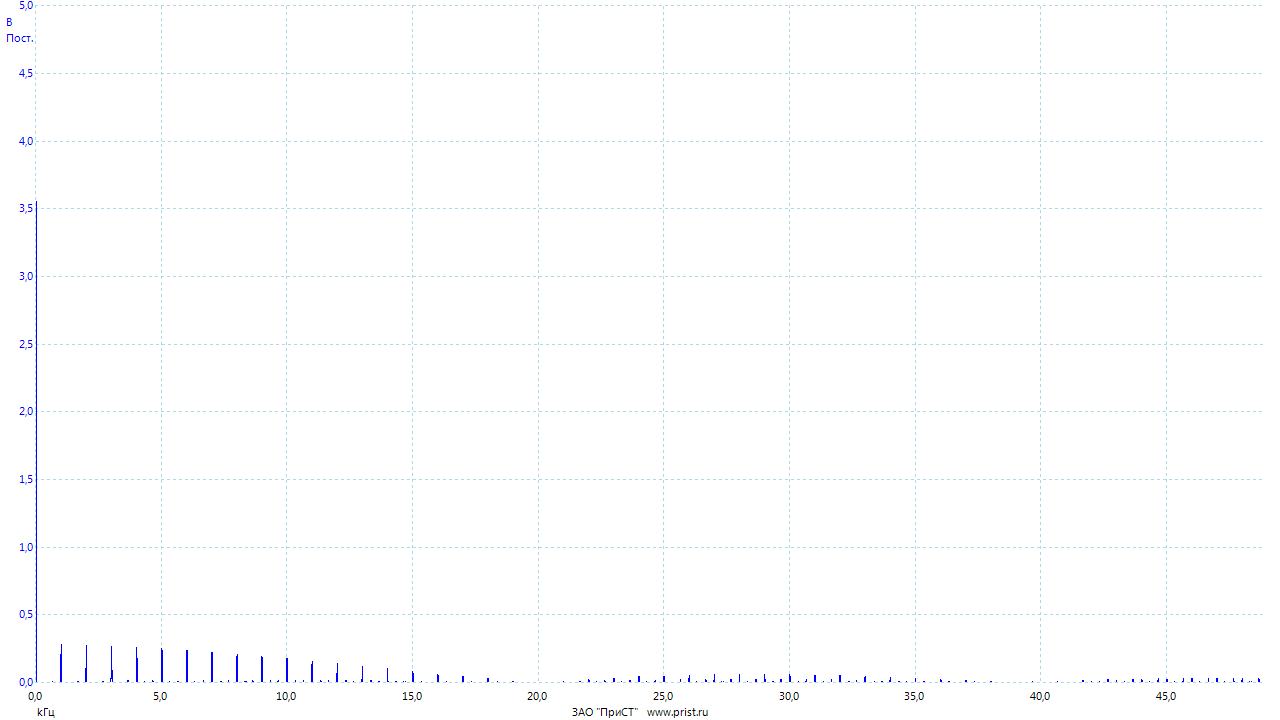
\includegraphics[width=\linewidth]{1кгц50мкс.png}
        
        {\small а) \(\nu_{\text{повт}} = 1\) кГц}
    \end{minipage}\hfill
    % Картинка 2
    \begin{minipage}[t]{0.5\textwidth}
        \centering
        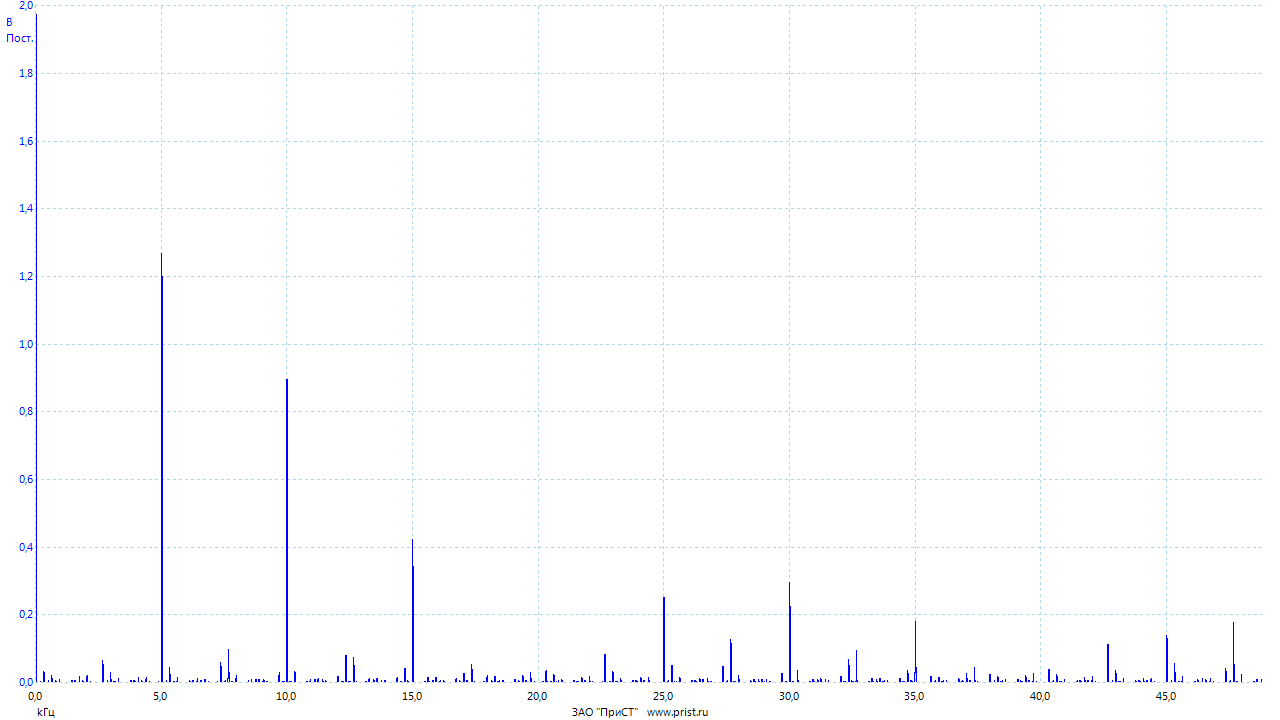
\includegraphics[width=\linewidth]{5кгц50мкс.png}
        
        {\small б) \(\nu_{\text{повт}} = 5\) кГц}
    \end{minipage}\hfill
    % Картинка 3
    \begin{minipage}[t]{0.5\textwidth}
        \centering
        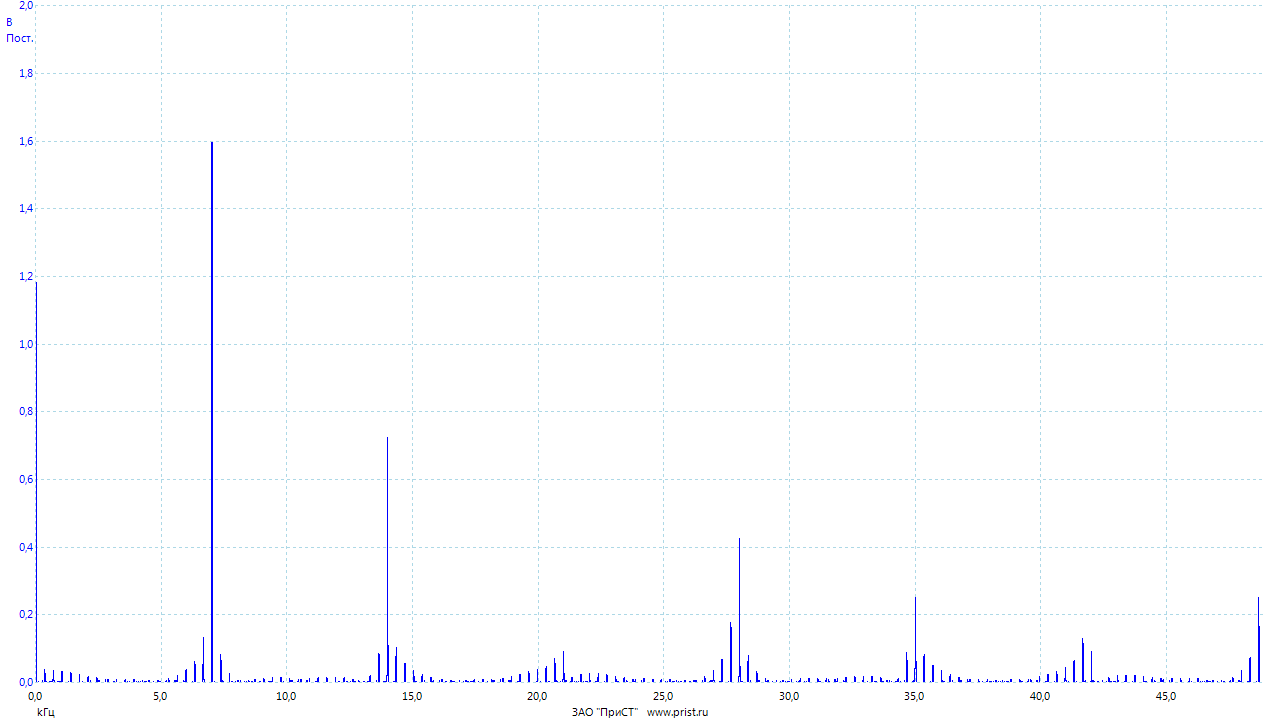
\includegraphics[width=\linewidth]{7кгц50мкс.png}
        
        {\small в) \(\nu_{\text{повт}} = 7\) кГц}
    \end{minipage}
    
    \vspace{0.2cm}
    \caption{Спектры прямоугольных импульсов при фиксированном \(\tau = 50\) мкс для различных частот повторения. Видно увеличение расстояния между гармониками \(\delta\nu\) с ростом \(\nu_{\text{повт}}\).}
    \label{fig:pulse_freq}
\end{figure}

\subsubsection*{б) Изменение длительности импульса \(\tau\) при фиксированной частоте повторения \(\nu_{\text{повт}} = 1\) кГц}

На рисунке представлены спектры сигнала при фиксированной частоте повторения \(\nu_{\text{повт}} = 1\) кГц и различных длительностях импульса: \(\tau = 50, 100, 150\) и \(200\) мкс.

\begin{itemize}
    \item При увеличении длительности импульса \(\tau\) ширина главного лепестка спектра (и всего спектра) \(\Delta\nu \sim 1/\tau\) \textbf{уменьшается}. Спектр становится более «узким» и сконцентрированным вблизи нулевой частоты.
    \item Положение нулей огибающей (частоты, на которых амплитуда гармоники обращается в ноль, \(\nu_k = k/\tau\)) смещается в сторону более низких частот. 
    \item Расстояние между соседними гармониками \(\delta\nu = \nu_{\text{повт}}\) остается неизменным, поскольку частота повторения зафиксирована (1 кГц).
\end{itemize}

% Используем [t] чтобы картинки прижимались к верху страницы, а не падали в самый низ
\begin{figure}[t]
    \centering
    % Верхний ряд
    \begin{minipage}[t]{0.48\textwidth}
        \centering
        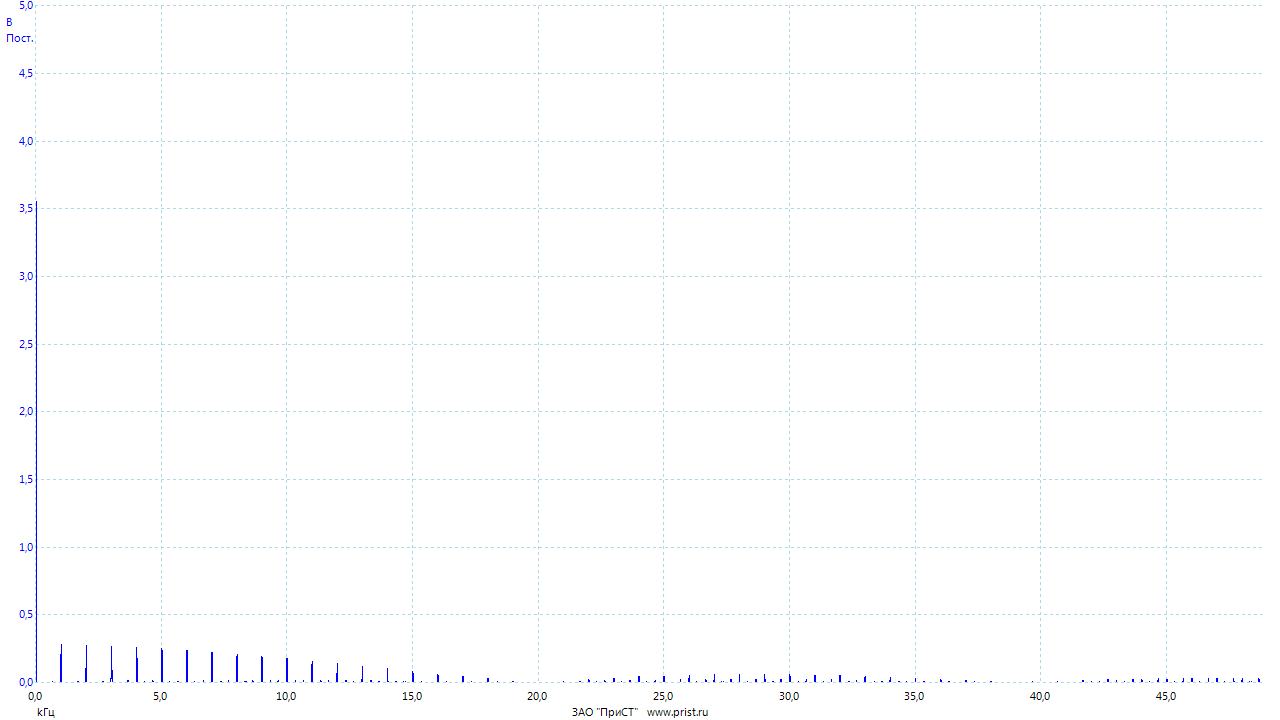
\includegraphics[width=\linewidth]{1кгц50мкс.png}
        
        {\small а) \(\tau = 50\) мкс}
    \end{minipage}\hfill
    \begin{minipage}[t]{0.48\textwidth}
        \centering
        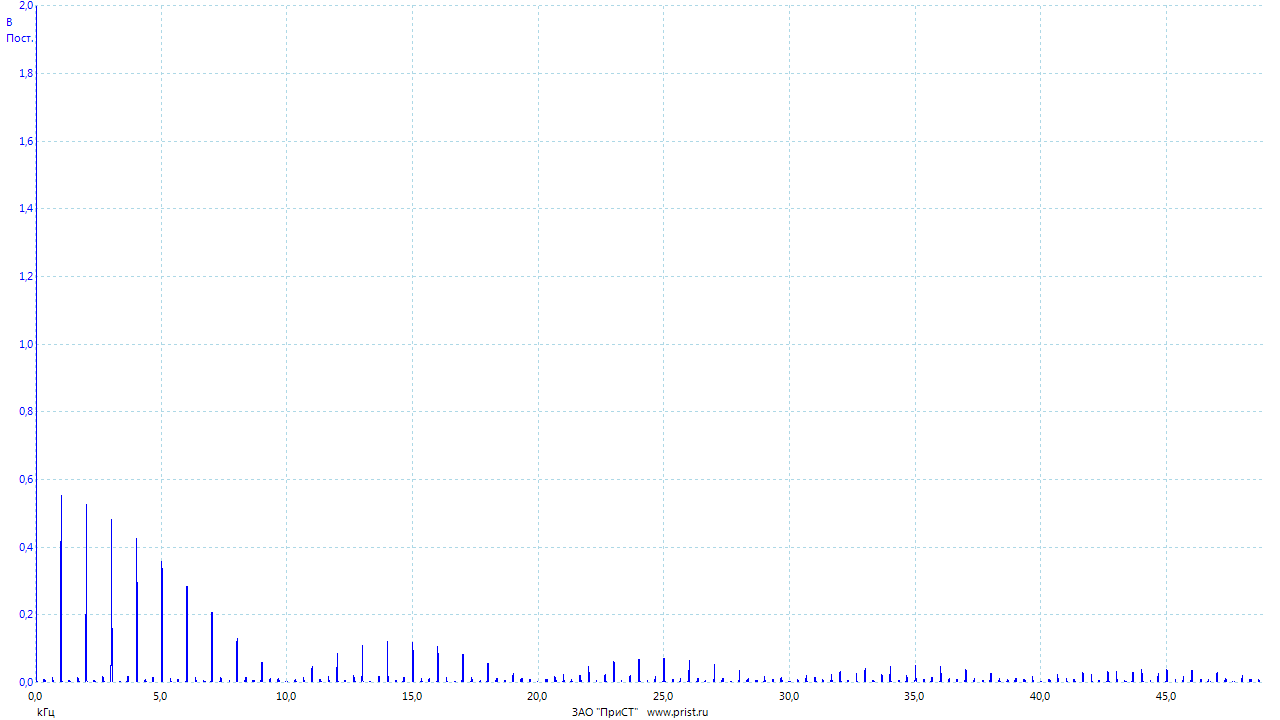
\includegraphics[width=\linewidth]{1кгц100мкс.png}
        
        {\small б) \(\tau = 100\) мкс}
    \end{minipage}
    
    \vspace{0.4cm}
    
    % Нижний ряд
    \begin{minipage}[t]{0.48\textwidth}
        \centering
        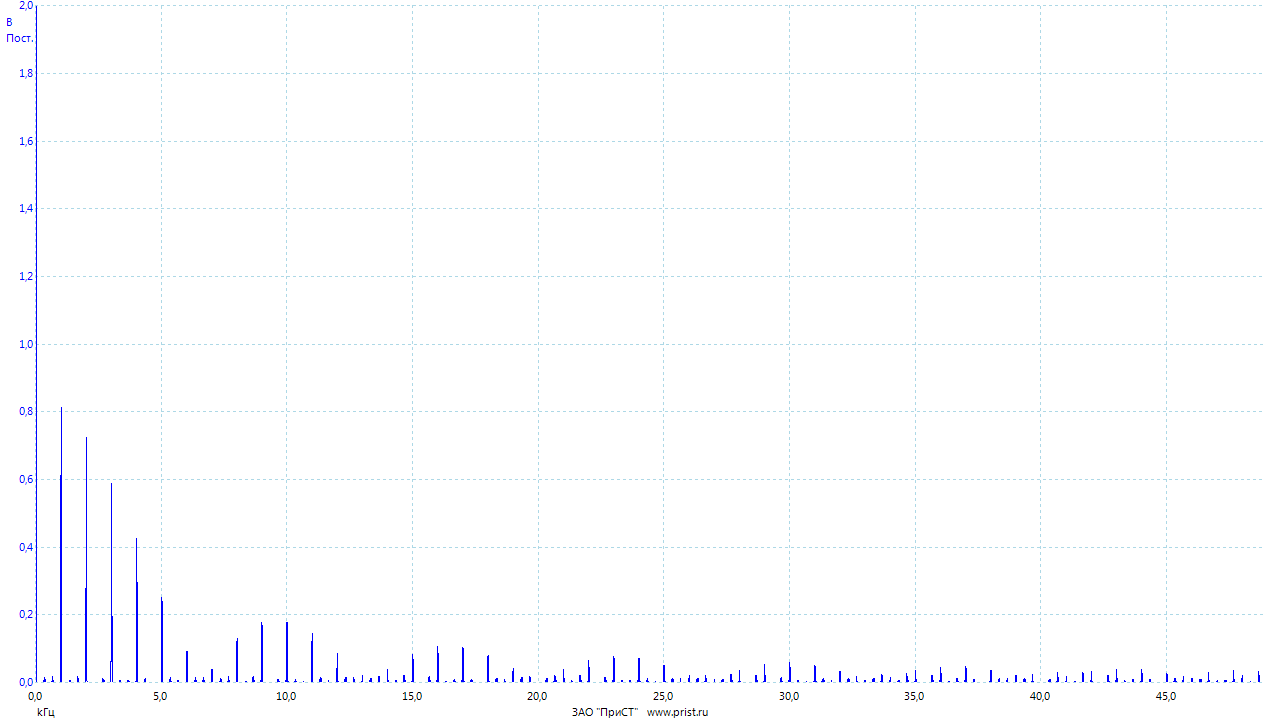
\includegraphics[width=\linewidth]{1кгц150мкс.png}
        
        {\small в) \(\tau = 150\) мкс}
    \end{minipage}\hfill
    \begin{minipage}[t]{0.48\textwidth}
        \centering
        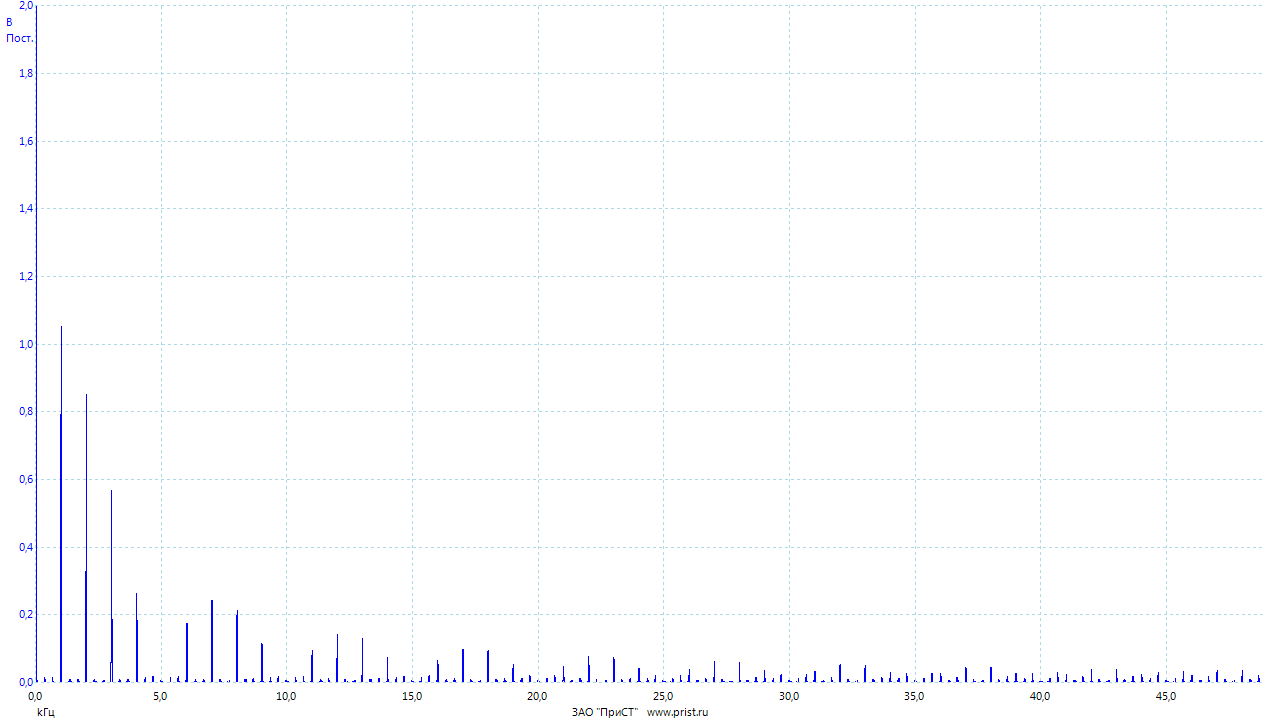
\includegraphics[width=\linewidth]{1кгц200мкс.png}
        
        {\small г) \(\tau = 200\) мкс}
    \end{minipage}
    
    \vspace{0.2cm}
    \caption{Спектры прямоугольных импульсов при фиксированном \(\nu_{\text{повт}} = 1\) кГц для различных длительностей \(\tau\). Наглядно видно сужение спектра \(\Delta\nu \sim 1/\tau\) при увеличении \(\tau\).}
    \label{fig:pulse_duration}
\end{figure}


\subsection*{ Измерение параметров спектра и сравнение с теорией}

Согласно методике, при фиксированных параметрах сигнала (\(\nu_{\text{повт}} = 1\) кГц, \(\tau = 50\) мкс) были измерены частоты \(\nu_n\) и амплитуды \(a_n\) первых нескольких спектральных гармоник. 

Теоретические значения частот рассчитываются как \(\nu_n = n/T = n\nu_{\text{повт}}\). Теоретические амплитуды гармоник определяются формулой:
\begin{equation}
|a_n|_{\text{теор}} = \frac{\tau}{T} \frac{\left|\sin(\pi \nu_n \tau)\right|}{\pi \nu_n \tau}
\end{equation}

В таблице \ref{tab:harmonics} представлены результаты измерений и их сравнение с теоретическим расчетом.

\begin{table}[htbp]
    \centering
    \caption{Сравнение экспериментальных и теоретических параметров спектра прямоугольных импульсов (\(\nu_{\text{повт}} = 1\) кГц, \(\tau = 50\) мкс)}
    \label{tab:harmonics}
    \begin{tabular}{|c|c|c|c|c|c|}
        \hline
        \multirow{2}{*}{\(n\)} & \multicolumn{2}{c|}{Частота, Гц} & \multicolumn{2}{c|}{\(|a_n/a_1|\)} & \(a_n^{\text{эксп}}\), В \\
        \cline{2-5}
        & \(\nu_n^{\text{эксп}}\) & \(\nu_n^{\text{теор}}\) & эксп. & теор. & \\
        \hline
        \(1\)  & \(1062\) & \(1000\) & \(1,000\) & \(1,000\) & \(1,055\) \\
        \(5\)  & \(5023\) & \(5000\) & \(0,337\) & \(0,904\) & \(0,355\) \\
        \(9\)  & \(9040\) & \(9000\) & \(0,091\) & \(0,702\) & \(0,096\) \\
        \(11\) & \(11040\) & \(11000\) & \(0,101\) & \(0,560\) & \(0,106\) \\
        \(15\) & \(15050\) & \(15000\) & \(0,063\) & \(0,290\) & \(0,066\) \\
        \(19\) & \(19060\) & \(19000\) & \(0,043\) & \(0,053\) & \(0,045\) \\
        \(20\) & \(20040\) & \(20000\) & \(\approx 0\) & \(0\) & \(\approx 0\) \\
        \(25\) & \(25050\) & \(25000\) & \(0,050\) & \(0,144\) & \(0,052\) \\
        \hline
    \end{tabular}
\end{table}

\paragraph{Анализ результатов:}
\begin{itemize}
    \item Измеренные частоты гармоник \(\nu_n^{\text{эксп}}\) с высокой точностью совпадают с теоретическими значениями \(\nu_n^{\text{теор}} = n \cdot \nu_{\text{повт}}\). Небольшое расхождение в пределах \(0,5-1\%\).
    \item Экспериментальное отношение амплитуд \(|a_n/a_1|\) качественно повторяет поведение теоретической огибающей спектра: амплитуда гармоник убывает с ростом \(n\). 
    \item На \(20\)-й гармонике (частота \(20\) кГц) наблюдается минимум (нуль огибающей), что теоретически ожидается при \(n = T/\tau = 1000/50 = 20\). Это подтверждает справедливость формулы для огибающей спектра прямоугольных импульсов.
\end{itemize}

\subsection*{ Измерение ширины спектра при изменении длительности импульса}

Согласно соотношению неопределённостей, ширина спектра прямоугольного импульса обратно пропорциональна его длительности: \(\Delta\nu \sim 1/\tau\). Для проверки этого утверждения при фиксированном периоде повторения \(T = 1\) мс (\(\nu_{\text{повт}} = 1\) кГц) изменялась длительность импульса \(\tau\) от \(50\) до \(200\) мкс. За полную ширину спектра \(\Delta\nu\) принималось расстояние от центра спектра (\(\nu = 0\)) до первой гармоники с нулевой амплитудой (первого нуля огибающей).

Результаты измерений представлены в таблице \ref{tab:width}.

\begin{table}[htbp]
    \centering
    \caption{Зависимость ширины спектра от длительности импульса (\(T = 1\) мс)}
    \label{tab:width}
    \begin{tabular}{|c|c|c|c|}
        \hline
        \(\tau\), мкс & \(1/\tau\), кГц & \(\Delta\nu^{\text{эксп}}\), кГц & \(\Delta\nu^{\text{теор}} \approx 1/\tau\), кГц \\
        \hline
        \(50\)  & \(20,0\) & \(20,0\) & \(20,0\) \\
        \(100\) & \(10,0\) & \(9,95\) & \(10,0\) \\
        \(150\) & \(6,67\) & \(6,7\)  & \(6,67\) \\
        \(200\) & \(5,0\)  & \(5,0\)  & \(5,0\) \\
        \hline
    \end{tabular}
\end{table}

\subsection*{ Измерение расстояния между гармониками при изменении периода повторения}

Согласно теории, расстояние между соседними гармониками в спектре периодического сигнала определяется исключительно периодом повторения: \(\delta\nu = 1/T\). Для проверки этого при фиксированной длительности импульса \(\tau = 100\) мкс изменялся период повторения \(T\) в диапазоне от \(1\) до \(5\) мс. Измерялось расстояние между соседними спектральными линиями \(\delta\nu\).

Результаты измерений представлены в таблице \ref{tab:delta}.

\begin{table}[htbp]
    \centering
    \caption{Зависимость расстояния между гармониками от периода повторения (\(\tau = 100\) мкс)}
    \label{tab:delta}
    \begin{tabular}{|c|c|c|}
        \hline
        \(T\), мс & \(1/T\), кГц & \(\delta\nu^{\text{эксп}}\), кГц \\
        \hline
        \(1,0\) & \(1,000\) & \(0,995\) \\
        \(2,0\) & \(0,500\) & \(0,472\) \\
        \(3,0\) & \(0,333\) & \(0,323\) \\
        \(4,0\) & \(0,250\) & \(0,248\) \\
        \(5,0\) & \(0,200\) & \(0,196\) \\
        \hline
    \end{tabular}
\end{table}

\subsection*{ Графическая проверка}


\begin{figure}[h!]
    \centering
    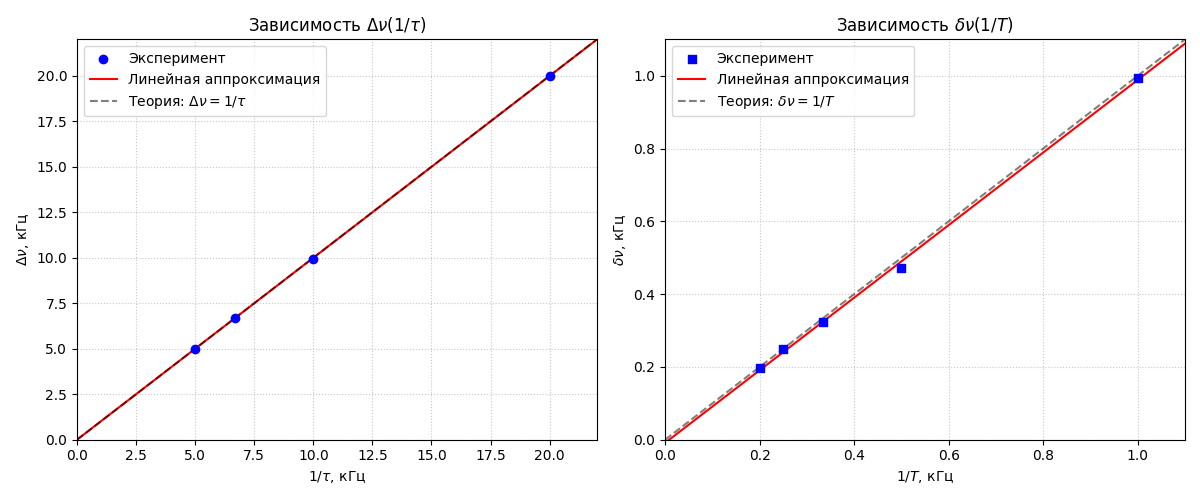
\includegraphics[width=1\textwidth]{uncertainty_plots.png}
    \caption{Проверка соотношений неопределённостей: а) зависимость ширины спектра от обратной длительности импульса; б) зависимость расстояния между гармониками от обратного периода повторения.}
    \label{fig:uncertainty}
\end{figure}

\paragraph{Анализ результатов:}
\begin{enumerate}
    \item Для \(\Delta\nu(1/\tau)\) получен наклон прямой \(k_1 = 0,9992\) и свободный член \(b_1 = 0,0038\) кГц. Коэффициент детерминации составил \(R^2 = 1,0000\). Наклон с высокой точностью совпадает с теоретическим значением \(1\), что подтверждает соотношение неопределённостей \(\Delta\nu \cdot \tau \approx 1\). 
    
    \item Для зависимости \(\delta\nu(1/T)\) получен наклон \(k_2 = 0,9971\) и свободный член \(b_2 = -0,0085\) кГц, \(R^2 = 0,9989\). Это подтверждает теоретическое положение о том, что расстояние между гармониками дискретного спектра определяется только периодом повторения сигнала.
\end{enumerate}

\subsection*{Б. Наблюдение спектра периодической последовательности цугов}



В ходе эксперимента изменялись параметры сигнала \(\nu_0\) и число периодов \(N\). На рисунке 4 представлены спектры цугов при различных параметрах.


\begin{figure}[htbp]
    \centering
    % Картинка 1
    \begin{minipage}{0.48\textwidth}
        \centering
        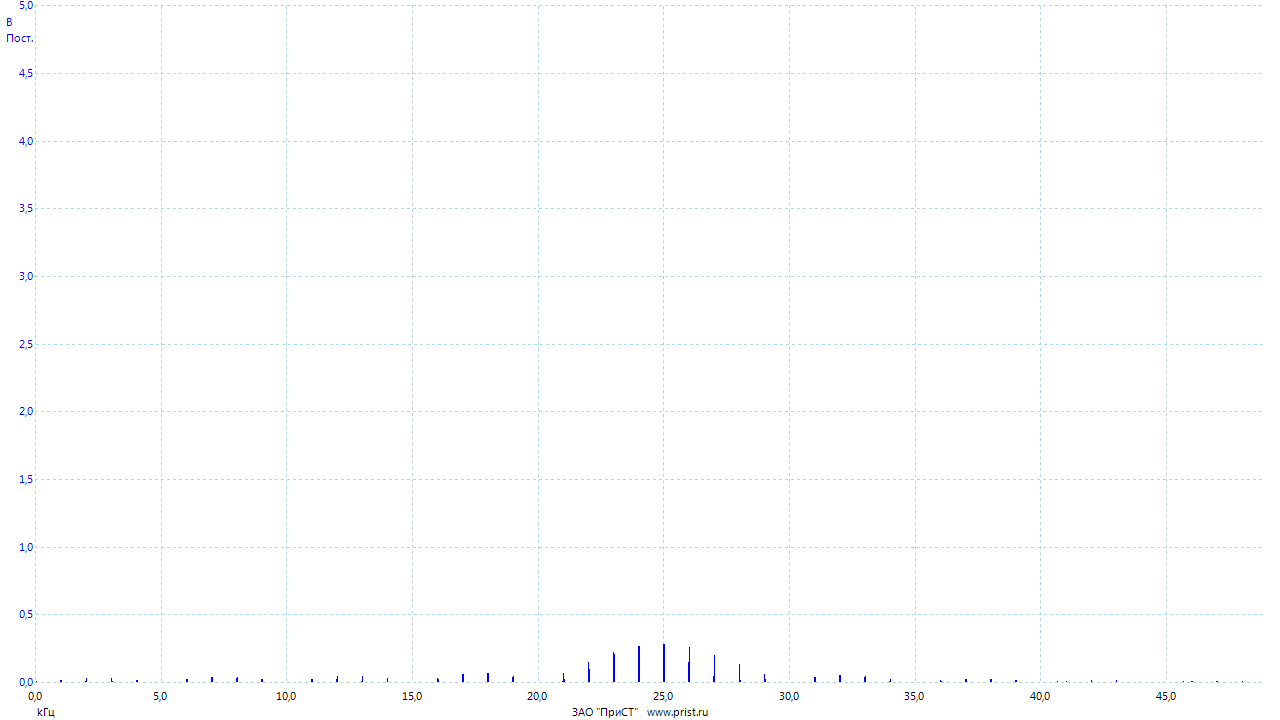
\includegraphics[width=\linewidth]{цуги 25кгц 1мс n5.png}
        
        {\small а) \(\nu_0 = 25\) кГц, \(N=5\)}
    \end{minipage}\hfill
    % Картинка 2
    \begin{minipage}{0.48\textwidth}
        \centering
        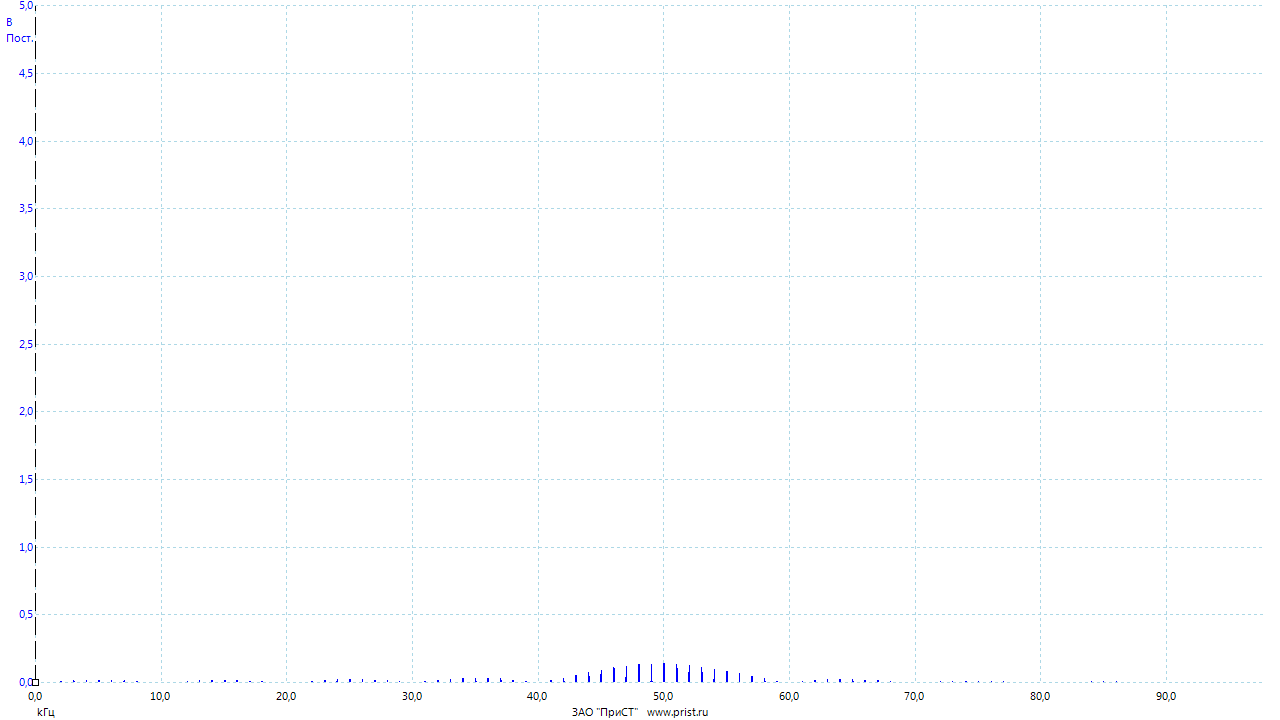
\includegraphics[width=\linewidth]{цуги 50кгц 1мс n5.png}
        
        {\small б) \(\nu_0 = 50\) кГц, \(N=5\)}
    \end{minipage}
    
    \vspace{0.3cm}
    
    % Картинка 3
    \begin{minipage}{0.48\textwidth}
        \centering
        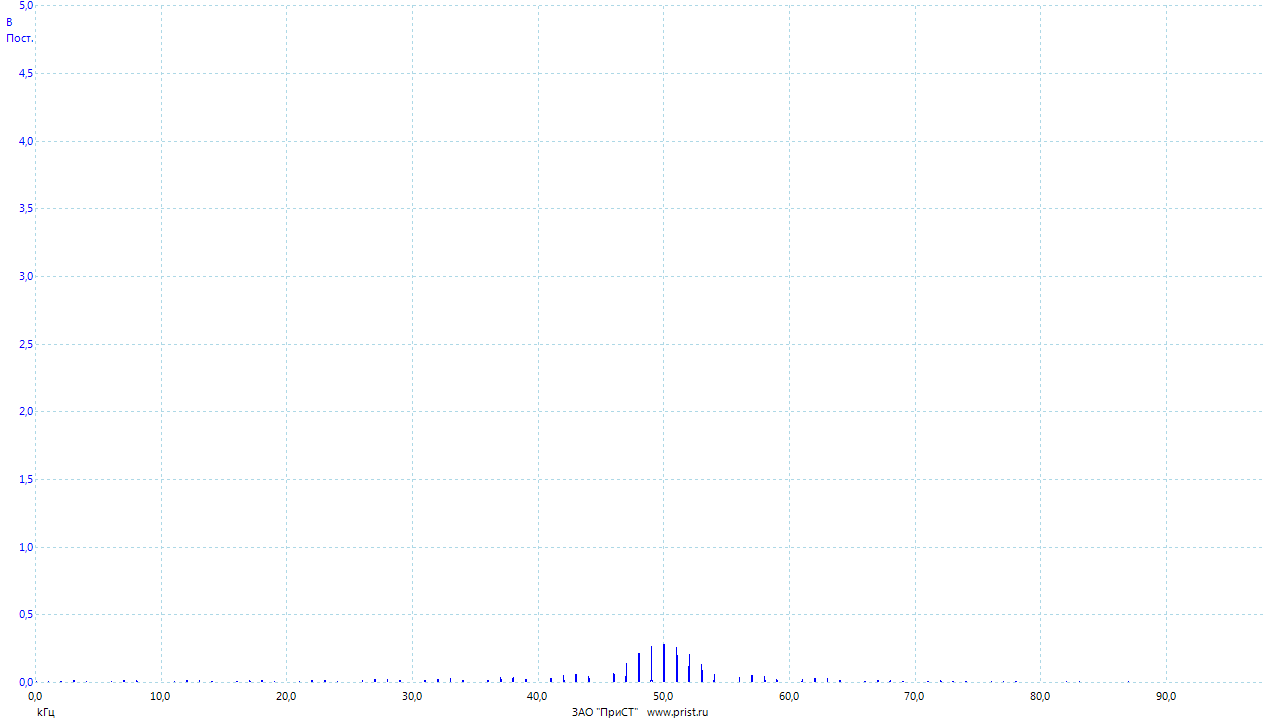
\includegraphics[width=\linewidth]{цуги 50кгц 1мс n10.png}
        
        {\small в) \(\nu_0 = 50\) кГц, \(N=10\)}
    \end{minipage}
    
    \vspace{0.2cm}
    % ЕДИНСТВЕННЫЙ И ГЛАВНЫЙ CAPTION
    \caption{Спектры периодической последовательности цугов при различных параметрах сигнала.}
    \label{fig:bursts}
\end{figure}

\subsubsection*{ Измерение параметров спектра и проверка теоремы смещения}

\begin{itemize}
    \item \textbf{Для \(N=5\)} (\(\nu_0 = 50\) кГц, \(\tau = 100\) мкс):
    \begin{itemize}
        \item Положение центра спектра: \(\nu_{\text{центр}} \approx 50,0\) кГц (совпадает с \(\nu_0\), что подтверждает теорему смещения).
        \item Расстояние между гармониками: \(\delta\nu \approx 1,0\) кГц (соответствует \(\nu_{\text{повт}}\)).
        \item Ширина главного лепестка: \(\Delta\nu \approx 20,0\) кГц (от \(\sim 40\) кГц до \(\sim 60\) кГц).
    \end{itemize}
    \item \textbf{Для \(N=10\)} (\(\nu_0 = 50\) кГц, \(\tau = 200\) мкс):
    \begin{itemize}
        \item Положение центра спектра: \(\nu_{\text{центр}} \approx 50,0\) кГц.
        \item Расстояние между гармониками: \(\delta\nu \approx 1,0\) кГц.
        \item Ширина главного лепестка: \(\Delta\nu \approx 10,0\) кГц (от \(\sim 45\) кГц до \(\sim 55\) кГц).
    \end{itemize}
\end{itemize}

\paragraph{Анализ результатов:}
\begin{enumerate}
    \item \textbf{Теорема смещения} подтверждается с высокой точностью: положение центра спектрального «сгустка» всегда совпадает с частотой заполнения цуга \(\nu_0\).
    \item \textbf{Соотношение неопределённостей} выполняется: при увеличении длительности цуга в 2 раза (от \(N=5\) до \(N=10\)) ширина его спектра уменьшается ровно в 2 раза (с \(\sim 20\) кГц до \(\sim 10\) кГц). Произведение \(\Delta\nu \cdot \tau\) остается постоянным.
    \item \textbf{Расстояние между гармониками} \(\delta\nu = 1\) кГц определяется периодом повторения цугов \(T = 1\) мс и не зависит от их внутренней структуры (несущей частоты и количества периодов).
\end{enumerate}






\end{document}
